\chapter{Подсистема Экосистемы OSTIS, обеспечивающая поддержку жизненного цикла умных домов}
\chapauthortoc{Андрушевич А.А.\\Войтешенко И.С.}

\label{chapter_smart_home}

\vspace{-7\baselineskip}

\begin{SCn}
	\begin{scnrelfromlist}{автор}
		\scnitem{Андрушевич А.А.}
		\scnitem{Войтешенко И.С.}
	\end{scnrelfromlist}
	
	\bigskip
	
	\scntext{аннотация}{В данной главе описан оригинальный подход к построению межотраслевой экосистемы интернета вещей и приложений умного дома через её семантическое представление на базе \textit{Технологии OSTIS}. Полученные результаты в будущем позволят повысить эффективность компонентного подхода к разработке приложений в интернете вещей, а также обеспечить возможность автоматической синхронизации различных версий компонентов, повышая их совместимость и согласованность.}
	\bigskip
	
	\begin{scnrelfromlist}{подраздел}
		\scnitem{\ref{sec_approach_analysis_for_smart_homes_design}~\nameref{sec_approach_analysis_for_smart_homes_design}}
		\scnitem{\ref{sec_proposed_approach}~\nameref{sec_proposed_approach}}
		\scnitem{\ref{sec_multicomponent_SH_model}~\nameref{sec_multicomponent_SH_model}}
		\scnitem{\ref{sec_SH_subsystems}~\nameref{sec_SH_subsystems}}
		\scnitem{\ref{sec_SH_tec_impl}~\nameref{sec_SH_tec_impl}}
		\scnitem{\ref{sec_SH_plans_and_tasks}~\nameref{sec_SH_plans_and_tasks}}
	\end{scnrelfromlist}
	
	\bigskip
	
	\begin{scnrelfromlist}{ключевое понятие}
		\scnitem{интернет вещей}
		\scnitem{веб вещей}
		\scnitem{умный дом}
		\scnitem{контекст}
		\scnitem{контекстно-зависимая система}
		\scnitem{REST API}
		\scnitem{ambient assisted living}
		\scnitem{MQTT}
		\scnitem{Node-RED}
		\scnitem{Yandex IoT Core}	
	\end{scnrelfromlist}
	
	\bigskip
	
	\begin{scnrelfromlist}{библиографическая ссылка}
		\scnitem{\scncite{Andrushevich2010}}
		\scnitem{\scncite{Paola2016}}
		\scnitem{\scncite{Kamilaris2018}}
		\scnitem{\scncite{Dobrescu2019}}
		\scnitem{\scncite{Standart2021}}
		\scnitem{\scncite{Stojkoska2017}}
		\scnitem{\scncite{Andrushevich2009}}
		\scnitem{\scncite{Biallas2017}}
		\scnitem{\scncite{Zhou2016}}
		\scnitem{\scncite{Beaudin2015}}
		\scnitem{\scncite{LCNR}}
	\end{scnrelfromlist}	
\end{SCn}

\section*{Введение в Главу~\ref{chapter_smart_home}}

Многоагентная и ситуационная (контекстная) обработка нашла широкое применение в приложениях интернета вещей, например в умном доме (cм. \scncite{Andrushevich2010}). Однако, несмотря на значительный прогресс последних лет в развитии отраслевых коммуникционных систем (ОКС) и автоматизированных систем управления (АСУ), по-прежнему актуальными остаются следующие проблемы:
\begin{textitemize}
	\item разнородность стандартов и технологий получения, хранения, обработки, передачи данных в приложениях интернета вещей;
	\item ограниченная отраслью функциональность ОКС;
	\item низкая адаптивность, совместимость и масштабируемость приложений.
\end{textitemize}

Таким образом, приходится констатировать отсутствие единого комплексного подхода к проектированию экосистемы межотраслевого универсального интернета вещей (ИВ).

\section{Анализ существующих подходов к созданию умных домов}
\label{sec_approach_analysis_for_smart_homes_design}

Отметим, что концепция повсеместного межотраслевого контекстно-зависимого безопасного интернета вещей быстро набирает популярность благодаря активно развивающейся конвергенции пакетов технологий, системных функций, платформ и услуг. Яркими примерами механизмов такой конвергенции являются становление и развитие таких общих системных функций в интернете вещей, как базовые службы / сервисы контекстной осведомленности, геолокации и информационной безопасности. Различные отрасли приложений интернета вещей также зачастую реализуют и используют схожие функциональные блоки, включая аутентификацию и авторизацию пользователей, гео-временную локализацию, обработку событий, контекстную осведомленность и многие другие. Например, научным сообществом уже опубликованы (см. \scncite{Paola2016}, \scncite{Kamilaris2018}, \scncite{Dobrescu2019}), результаты разработки базовых технологий и алгоритмов для получения и предоставления информации о гео-временном местоположении и контексте. На самом деле, видение повсеместного всепроникающего интернета вещей включает в себя не только множество технологий, но и динамические изменения окружающей среды и виртуальное информационное окружение (пространство) пользователей. Сбор и использование контекстной информации выходит за рамки обычных приложений с замкнутым циклом, которые используют только простую информацию о местоположении. Например, универсальная гео-временная информация успешно модернизирует приложения интернета вещей в таких отраслях, как дом, офис, промышленность, торговля, транспорт, здравоохранение, города.

\section{Предлагаемый подход к созданию умных домов}
\label{sec_proposed_approach}

В рамках данной работы предлагается взять за основу общеизвестные компоненты и библиотеки Технологии OSTIS (cм. \scncite{Standart2021}) для формализации описания предметной области экосистемы интернета вещей. Системы, разрабатываемые на основе Технологии OSTIS, названы \textit{ostis-системами}. В основе \textit{Технологии OSTIS} лежит универсальный способ смыслового представления (кодирования) информации в памяти интеллектуальных компьютерных систем, названный \textit{SC-кодом}. Таким образом может быть достигнута лучшая конвергенция разнородных стандартов и технологий интернета вещей, которая поспособствует межотраслевой интеграции ОКС и АСУ в единую экосистему.

Итак, дадим следующие определения рассматриваемой предметной области интернета вещей в \textit{SC-коде}:
\begin{SCn}
\scnheader{интернет вещей}
\scnidtf{Множество физических объектов, подключенных к интернету и обменивающихся данными. Термин «интернет вещей» был впервые употреблен в 1999 году Кевином Эштоном, предпринимателем и соучредителем центра Auto-ID Labs (распределённая исследовательская группа в области радиочастотной идентификации и новых сенсорных технологий) при Массачусетском технологическом институте MIT}
\scnidtf{Концепция сети передачи данных между физическими объектами («вещами»), оснащёнными встроенными средствами и технологиями для взаимодействия друг с другом или с внешней средой}
\end{SCn}

\begin{SCn}
\scnheader{веб вещей}
\scnidtf{Глобальная сеть веб-страниц, автоматически сгенерированных и автоматически считываемых встроенными в физические объекты (парковка, тротуарная плитка, окна, двери, детская игрушка, посуда, одежда, почва и т.д.) вычислительными устройствами. Для веба вещей характерна конвергенция и интеграция с технологиями искусственного интеллекта}
\scnidtf{Подход от W3C по использованию веб-технологий в интернете вещей с целью устранения фрагментации в стандартах разработки интернета вещей}
\end{SCn}

\begin{SCn}
\scnheader{Контекстно-зависимая информационная система}
\scnidtf{Информационная система, использующая понятие контекста для предоставления имеющей отношение персонифицированной динамической информации и / или услуг пользователю, где степень отношения зависит от текущей среды окружения, интересов, задач, намерений и действий пользователя}
\end{SCn}

\begin{SCn}
\scnheader{Прикладной программный интерфейс с передачей репрезентативного состояния}
\scnidtf{Концепция построения распределённого приложения по типу клиент-сервер, в которой каждый запрос (REST-запрос) клиента к серверу содержит в себе исчерпывающую информацию о желаемом ответе (репрезентативном состоянии) сервера без необходимости хранения информации о состоянии клиента (клиентской сессии)}
\end{SCn}

На основе многолетнего профессионального опыта авторов можно утверждать, что организация универсального типового межотраслевого (или "горизонтального") способа технологической реализации системной архитектуры и приложений в интернете вещей может быть представлена в виде трех потоков разработки, каждый из которых посвящен реализации одной системной платформы интернета вещей. Эти 3 фундаментальные независимые от приложений платформы вместе образуют типовую архитектурную платформу интернета вещей, которая интегрируется во взаимосвязанную гетерогенную систему подсистем интернета вещей, предлагая разработчикам приложений общие функциональные возможности  и оставляя разработчикам больше времени для концентрации на бизнес-логике их приложений.

\begin{figure}[H]
	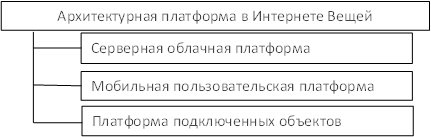
\includegraphics[scale=0.7]{/images/part7/chapter_smart_home/IoT-Architecture-Platform.png}
	\caption{Архитектура платформы IoT}
	\label{fig:iot}
\end{figure}

\textit{Серверная облачная платформа}, обладающая высокими вычислительными ресурсами и большими объёмами памяти, в наибольшей степени управляет всей системой интернета вещей. \textit{Платформа для мобильных устройств} отвечает за представление результирующей и полезной информации пользователям. \textit{Платформа подключенных объектов}, объединяет сенсорную информацию об окружающей среде и способна выполнять простые действия через подключенные объекты.

Опишем указанные выше платформы подробнее:
\begin{textitemize}
    \item платформа Smart Server: совокупность различных серверов для обеспечения API строительных блоков в облаке для интеграции приложений и сервисов. Данная платформа обладает высокими вычислительными возможностями, большим количеством ресурсов памяти и может взаимодействовать с любыми стандартами. Можно считать вычислительные ресурсы и возможности неограниченными. Её роль заключается в сборе, агрегировании и / или интерпретации контекстно-зависимой информации, поступающей от подключенных узлов приложений ИВ, чтобы сделать ее эффективной и имеющей смысл (потребительскую ценность) для пользователей мобильных устройств. Она также предоставляет разработчикам приложений API-интерфейсы локальных или удаленных универсальных базовых компонент, реализующих функциональность серверной стороны всех приложений, например: обработку и аналитику больших данных, сложную обработку событий, механизм локализации, фреймворк контекстного управления, профиль пользователя и модель поведения пользователей, политики безопасности, контроль доступа (включая регистрацию пользователей, аутентификацию и схему доверия). Наиболее распространёнными примерами платформы Smart Server являются Yandex.Cloud, Amazon Web Services (AWS), Microsoft Azure, Google Cloud, Cisco IoT Cloud Connect, SAP, Oracle IoT, ThingsBoard, SiteWhere, Predix IoT, Thinger.io, Ubidots;
    \item платформа Smart Mobile: эталонная платформа для мобильных приложений, обеспечивающая функциональность на мобильных устройствах для всех приложений ИВ. Мобильные устройства наиболее часто принадлежат конечным пользователям-людям. Общими функциями мобильных клиентов являются: общие компоненты пользовательских интерфейсов, профилирование пользователей, аутентификация и авторизация, информационная безопасность (конфиденциальность), поиск и обнаружение интеллектуальных серверов, связь с серверными компонентами, получение уведомлений от серверов, "локальные" алгоритмы добычи данных (толстый клиент). Данная платформа предоставляет приложениям ИВ возможность использовать необходимую им контекстную информацию, не беспокоясь о том, каким образом эта контекстная информация добывается. Мобильная платформа может взаимодействовать как с платформой Smart Server, так и непосредственно с некоторыми подключенными узлами ИВ. В заключение мобильная платформа ИВ отвечает за последний этап формирования потребительской ценности через мультимедийное представление / вывод последовательной и интересующей пользователей информации. Наиболее распространёнными примерами платформы Smart Mobile являются Zetta, HP Enterprise Universal, Carriots, ThingsBoard, ThingWorx, Xively. Для сокращения времени разработки мобильных приложений часто используются так называемые гибридные приложения, код которых адаптируется при помощи фреймворков сразу под несколько мобильных аппаратных платформ. Таикими наиболее популярными фреймворками являются: PhoneGap, Rhodes, Appcelerator, Xamarin, Ionic, Appy Pie, Native Script.
    \item платформа Smart Object: интеграция различных шлюзов, сетевых концентраторов и связанных с ними технологий подключенных объектов. Подключенные объекты могут воспринимать физические данные окружающей среды (температура, давление, освещённость, влажность, вибрация и т.д.) через датчики или быть исполнительными механизмами (выключатель, электропривод, электромагнит и т.д.). Передача данных как правило происходит через маломощные коммуникационные стандарты связи. Такие устройства также могут быть оснащены "легковесной" операционной системой. Такие устройства очень разнородны и могут работать очень по-разному. Однако, все особенности реализации подключённых объектов (вещей) должны быть скрыты от других устройств, чтобы обеспечить однородный способ общения с другими компонентами системы, независимо от того, какие данные они воспринимают или как они устроены. Следовательно, единый объектный программный интерфейс является ключевым моментом для того, чтобы иметь возможность легко интегрировать различные шлюзы, обеспечивающие доступ к различным подключённым объектам через одни и те же стандарты, не требуя от разработчиков приложения ИВ знания сложности взаимосвязи объектов со шлюзом и того, какие функциональные возможности (сбор данных или приведение в действие) выполняются на этих объектах. Данная платформа обладает общими функциями, такими как: обнаружение объектов, безопасность и управление. Наиболее распространёнными примерами платформы Smart Object являются open source IoT Kaa, Arduino, Flutter, Qualcomm’s IoT Development Kit, Particle.io, ESP8266, Intel Edison, Raspberry Pi, Beagle Bone..
\end{textitemize}

Описываемые в данной работе предметные области разрабатывались на основе  % субъектно-объектных воздействий, предложенной в работе В. Мартынова и его учеников \cite{Martynov1974}, \cite{Martynov1977}, \cite{Martynov1984}, \cite{Hardzei2017}, \cite{Hardzei2020}.

\section{Многокомпонентная модель умных домов}
\label{sec_multicomponent_SH_model}

Данный раздел посвящён теоретическому определению универсальной многокомпонентной модели типового приложения интернета вещей для платформ из предыдущего подраздела. Описание для "канонической" или "классической" архитектуры приложения интернета вещей, состоящей из облака или серверных мощностей, различных протоколов предачи данных, пользовательских устройств (ПК, ноутбуки, планшеты, телефоны, встраиваимые пользовательские интерфейсы в любые устройства), любого рода датчики по сбоду данных и любого "устройства-исполнители-руки". Учитывая особенности и свойства трех частей горизонтальной платформы (Smart Server, Smart Mobile и Smart Object), а также характеристики приложений интернета вещей, предлагается следующее универсальное древовидное представление многокомпонентной модели архитектуры приложения в интернете вещей.

Все компоненты и параметры данной древовидной иерархической модели приведены в качестве примера и могут изменяться в конкретных приложениях ИВ.

(0) Приложение Интернета Вещей S = A * B * C

(1) Интеллектуальная Серверная Платформа A = D * E

(1.1) Контроль Доступа D = G * H * I

    (1.1.1) Регистрация G: G1 (Пользователи), G2 (Машины)

    (1.1.2) Аутентификация H: H1 (Периодическая), H2 (По Требованию)

    (1.1.3) Схема доверия I: I1 (Управляемая приложениями), I2 (Управляемая политикой), I3 (Управляемая профилем), I4 (Управляемая рисками)

(1.2) Обработка Данных E = J * K * L

    (1.2.1) Контекстное управление J: J1 (Управляемое событиями), J2 (Опрос)

    (1.2.2) Обработка потока K: K1 (Оффлайн), K2 (Полу-онлайн), K3 (Онлайн)

    (1.2.3) Хранение Данных L: L1 (Простое), L2 (Иерархическое), L3 (Структурированное), L4 (Динамическое)

(2) Интеллектуальная Мобильная Платформа B = M * Phi

(2.1) Общие Характеристики Мобильности M = O * P

    (2.1.1) Основной тип траффика данных O: O1 (Мультимедиа), O2 (Восприятие/считывание), O3 (Управление), O4 (Хорошо сбалансированный)

    (2.1.2) Информация о местоположении P: P1 (Режим включения/выключения), P2 (На основе точности)

(2.2) Пользовательский Интерфейс Phi = R * F

    (2.2.1) Пользовательский интерфейс R: R1 (Один носитель), R2 (Мультимедиа), R3 (Адаптивный)

    (2.2.2) Доставка контента F: F1 (На основе услуг), F2 (На основе устройств)

(3) Платформа Интеллектуального Объекта C = Q * T

    (3.1) Общие Характеристики Узла Q = W * V * U

    (3.1.1) Источник Питания W: W1 (Пассивный), W2 (Активный)

    (3.1.2) Физическое взаимодействие V: V1 (Считывание), V2 (Действие), V3 (Комбинированное)

    (3.1.3) Шифрование U: U1 (Да), U2 (Нет)

(3.2) Связность T = X * Y * Z

    (3.2.1) Носитель X: X1 (Беспроводной), X2 (Проводной)

    (3.2.2) Тип сети Y: Y1 (Сетка), Y2 (Точка-точка)

    (3.2.3) Конфигурация Z: Z1 (Адаптивная), Z2 (Статическая)

На основе предложенной древовидной многокомпонентной модели экосистемы интернета вещей могут быть реализованы такие приложения интернета вещей, как умный дом, офис, промышленность, торговля, транспорт, здравоохранение, умные города.

Остановимся на популярном приложении умный дом и опишем его функции более подробно.

\section{Подсистемы умного дома}
\label{sec_SH_subsystems}

Среди функциональных задач, реализуемых в виде компонентов/приложений при проектировании и разработке программно-аппаратного обеспечения «умного дома» (cм. \scncite{Stojkoska2017}), типичными являются:
\begin{textitemize}
\item задача доступа к жилое помещение;
\item задача наблюдения за одинокими пожилыми людьми (cм. \scncite{Andrushevich2009}, \scncite{Biallas2017});
\item задача управления освещенностью жилища;
\item задача управления энергопотреблением и энергоэффективностью (cм. \scncite{Zhou2016}).
\end{textitemize}

Таким образом, функциональная классификация приложений умного дома может быть определелена с использованием SC-кода следующим образом:
\begin{SCn}
\scnheader{Приложение умного дома}
\scnidtf{обособленный программно-аппаратный комплекс, работающий согласно функциональным требованиям}
\scnrelfrom{разбиение}{Разбиение класса приложений умного дома по функциональности}
\begin{scnindent}
\begin{scneqtoset}
\scnitem{приложение управления физическим доступом}
    \begin{scnindent}
    \scnsuperset{функциональность контроля и управления состоянием всех традиционных и эвакуационных входов и выходов помещения}
    \end{scnindent}
\scnitem{приложение наблюдения за одинокими пожилыми людьми}
    \begin{scnindent}
    \scnsuperset{функциональность по обеспечению бытовой безопасности одиноких пожилых людей}
    \end{scnindent}
\scnitem{приложение управления освещенностью жилища}
    \begin{scnindent}
    \scnsuperset{функциональность контроля и управления состоянием источников естественного и искусственного освещения}
    \end{scnindent}
\scnitem{приложение управления энергопотреблением и энергоэффективностью}
    \begin{scnindent}
    \scnsuperset{функциональность контроля и управления потребления всех видов ресурсов и энергии}
    \end{scnindent}
\end{scneqtoset}
\end{scnindent}
\end{SCn}

Далее более детально опишем функциональность вышеуказанных приложений умного дома.

\subsection{Подсистема доступа в жилое помещение}
Ключевой задачей такой системы является идентификация людей, которые подходят к двери помещения, и корректная обработка ее результатов: если подошедший к двери человек должен иметь доступ к помещению, дверь открывается автоматически, в противоположном же случае система предлагает поговорить с жителями дома или квартиры. При этом желательно, чтобы система умела определять, находится ли кто-то из жителей дома. Если дома никого нет, то система должна сообщить посетителю, что зайти сейчас он не может.

С точки зрения устройств система оснащена камерой, а также лампами для освещения. Камера включается по датчику движения, причем также включается и освещение, если окружающая среда слишком темная для работы камеры. Система пытается распознать посетителя по снимкам с камеры.

В дополнение к данным камеры, система также имеет в своем распоряжении данные о местоположении жителей. Если по данным геолокации никого нет дома, то система отклоняет посетителей. Также для пользователя предусмотрена возможность включить такой режим вручную. Это может быть полезно, например, если в какой-то период времени жителей не должны беспокоить.

Система также должна содержать графический пользовательский интерфейс, через который можно как наблюдать за выбранными показателями и состоянием устройств, так и управлять поведением системы. Кроме того, через пользовательский интерфейс жители могут получать уведомления о том, что кто-то пытается войти в помещение.

Таким образом, можно выделить следующие функциональные требования к системе:

\begin{enumerate}
	\item Система позволяет задать несколько профилей жителей таким образом, чтобы их можно быть идентифицировать на входе.
	\item При положительной идентификации система открывает дверь автоматически.
	\item В состоянии по умолчанию камера и освещение выключены, однако они должны включаться по необходимости.
	\item Система может определить, находится ли кто-либо из жителей дома или нет. В случае, если никого нет дома, система должна сообщить посетителю об этом. В противном случае система должна предложить поговорить с людьми внутри помещения.
	\item Система также должна поддерживать режим «Не беспокоить». Поведение системы при этом соответствует случаю, когда в помещении никого нет.
	\item Система должна уведомлять жителей о посетителях.
\end{enumerate}

В дополнение к функциональным требованиям к системе также были разработаны следующие нефункциональные требования:

\begin{enumerate}
	\item Система может распознавать до 10 различных профилей жителей.
	\item Система должна корректно реагировать на сигналы устройств, даже если произошел разрыв соединения.
	\item Допустимо также ручное управление, в частности, использование ключа для того, чтобы открыть дверь.
	\item Поддерживается расширение системы большим количеством устройств.
\end{enumerate}

\subsection{Подсистема наблюдения за одинокими пожилыми людьми}

В условиях снижающейся рождаемости доля пожилых людей в обществе растет, в то время как доля людей трудоспособного возраста снижается. Пожилые люди часто нуждаются в помощи с заботой о здоровье, свободном перемещении и в случае нежелательных происшествий. Благодаря использованию технологий интернета вещей, такие люди могли бы жить в большей безопасности и комфорте. Сфера интернета вещей, связанная с наблюдением за пожилыми людьми, также называется AAL (ambient assisted living, проживание с фоновым сопровождением).

В \scncite{Andrushevich2009} были выделены следующие сферы применения технологий IoT:

\begin{enumerate}
	\item информационная 	помощь 	(легкодоступность 	всей 	необходимой информации),
	\item умное ситуационное поведение (среда должна узнавать типичные шаблоны поведения и предлагать соответствующую помощь),
	\item предсказание нежелательных событий (распознавание таких ситуаций на основании поведенческих и физиологических показателей, а также применение превентивных мер),
	\item распознавание нежелательных ситуаций и реакция на них,
	\item безопасность (защита от вторжений с использованием авторизационных и аутентификационных механизмов),
	\item конфиденциальность (минимизация вмешательства в личную жизнь).
\end{enumerate}

Для удовлетворения указанных потребностей система может полагаться как на исторические, так и получаемые в реальном времени данные. Выделяют две группы датчиков. Данные об окружающей среде исходят от датчиков окружения, например, температуры, движения. Данные о поведении и состоянии человека исходят от носимых датчиков. В системе также могут присутствовать устройства обратной связи для визуального и голосового уведомления о различных событиях. Современные технологии беспроводной связи позволяют создавать надежную, легкую в установке и недорогую инфраструктуру для передачи данных.

Центральным для систем AAL являются сбор и хранение данных о поведении пользователя, выделение шаблонов и определение нежелательных ситуаций на основании отклонений от них. Состояние пользователя может быть определено на основе данных от нескольких датчиков, расположенных в жилище (cм. \scncite{Biallas2017}).

Среди нежелательных ситуаций особо отметим падения. Одним из способов распознавания падений является совместное использование носимого датчика ускорения и атмосферного давления. В случае неожиданного ускорения система дважды считывает данные о давлении, на основании которых делает вывод о положении тела человека (cм. \scncite{Andrushevich2009}).

С точки зрения моделирования таких систем можно выделить три категории показателей. К физическим аспектам относятся как условия внешней среды, так и параметры здоровья человека. В связи с непрерывной природой этой категории наиболее естественным представляется метод системной динамики в сочетании со стохастическим моделированием для учета роли случайности. С другой стороны, дискретно-событийное моделирование позволяет учесть появляющиеся события, например, падения. Наконец, спонтанное поведение пользователя наилучшим образом моделируется с помощью агентного метода.

\subsection{Подсистема для управления освещенностью жилища}
Примерные функциональные требования к приложению: при входе в помещение свет загорается, среагировав на движение, а через 10 секунд после выхода из помещения свет отключается. Яркость освещения должна корректироваться с учетом уровня уличного освещения, проникающего в жилище. Кроме того, освещение с 23-00 до 6-00 утра должно работать в режиме ночника, с пониженной яркостью.

\subsection{Подсистема управления энергопотреблением и энергоэффективностью}
В связи с нарастающим энергетическим кризисом и неадекватностью традиционных централизованных энергосистем новым вызовам появилась новая модель: гибридное распределенное производство энергии со значительным вкладом возобновляемых источников энергии. Такая модель также характеризуется двунаправленным потоком информации и электричества. Существуют решения на всех этапах производства энергии, однако на стороне потребителя основным является направление интернета вещей, в частности, домашней автоматизации. Такие системы получили название HEMS (home energy management system, система управления энергопотреблением для жилых домов) (cм. \scncite{Stojkoska2017})

К системам управления энергией предъявляют следующие требования (cм. \scncite{Zhou2016}):

\begin{enumerate}
	\item Система собирает в реальном времени данные о потреблении и получении энергии, а также о состоянии устройств.
	\item Система сохраняет и анализирует исторические данные.
	\item Система управляет устройствами в своих рамках таким образом, чтобы обеспечить оптимальное энергопотребление.
	\item Пользователь имеет возможность управления устройствами напрямую и удаленно.
	\item В случае возникновения нежелательных ситуаций система предупреждает пользователя.
\end{enumerate}

Рассмотрим выбор метрик для оценки работы систем управления энергопотреблением.

Среда работы систем управления энергопотреблением --- жилое помещение, домохозяйство, даже офисное или производственное здание --- приводит к многоцелевому характеру таких систем [6], то есть к необходимости нахождения компромисса между несколькими задачами. В то время как глобальной целью всегда является повышение эффективности использования энергии, на ее достижения налагаются ограничения, в частности, по комфорту пользователей. Кроме того, формулировка конкретной задачи может разниться в зависимости от контекста: снижение выбросов, денежная экономия, балансировка нагрузки на энергосистему — вот некоторые возможные направления.

Цели управления потреблением энергии могут быть выражены через стоимость. Хотя наиболее очевидным и преобладающим фактором является цена потребляемой энергии, в общую формулу расчета также могут включаться такие факторы, как затраты на начальную установку системы, штраф за вклад в общую нагрузку, прогнозируемый износ оборудования, налог на выбросы парниковых газов (cм.\scncite{Beaudin2015}). Таким образом, система может следовать единой цели — снижение получаемых по этой формуле денежных затрат. Выбор корректного соотношения может представлять сложность, если нет устоявшихся денежных значений для некоторых целей.

Основная задача из тех, которые сложно представить в денежном эквиваленте, — это комфорт пользователей, то есть их неудобства, связанные с качеством услуг, предоставляемых при доставке энергии. Система не должна приводить к значительному изменению их образа жизни. Для оценки влияния системы на комфорт пользователей могут использоваться различные штрафные функции: ограничения по значению, отклонение, штраф за отсутствие сервиса (cм. \scncite{Beaudin2015}). Иначе говоря, если стоимость представляет собой некоторое соотношение, которое требуется минимизировать, то требования по комфорту налагают ограничения на возможные стратегии.

Описанные выше соображения могут применяться в тестировании общих подходов к оптимизации потребления энергии. Например, может потребоваться оценить выгоды от добавления того или иного устройства и сравнить их с ценой приобретения и установки, или же выбрать из нескольких разрабатываемых алгоритмов наилучший.

С точки зрения конечного пользователя к системе могут предъявляться такие требования, как доступ к историческим данным и тенденциям, возможность удаленного управления устройствами, предупреждение о нежелательных ситуациях  (cм. \scncite{Zhou2016}). Конфиденциальность данных, надежность и эффективность системы также играют роль в оценке ее качества. Подобные требования скорее характерны для продуктов практической направленности, предназначенных для прямого использования по назначению, а не исследовательских прототипов.

\section{Элементы технической реализации умных домов}
\label{sec_SH_tec_impl}
Проектирование и программная реализация указанных компонентов/приложений осуществлялось с помощью инструмента  визуального программирования Node-RED  в сочетании с использованием облачных технологий, в частности, Yandex IoT Core  или AWS IoT Core. Node-RED  — это инструмент потокового программирования для соединения аппаратных устройств, API и онлайн сервисов. Их совместное позволяет создавать прототипы систем интернета вещей без использования реальных устройств, что позволяет проработать архитектуру системы до ее физической реализации.  Одним из немаловажных преимуществ Node-RED является то, что с помощью этого инструмента возможно создать простой прототип системы в той же среде, в которой ведется или будет вестись основная разработка. Такой подход значительно упрощает разработку. Кроме того, Node-RED также предоставляет средства для простой визуализации получившейся системы, что позволяет создать прототип графического интерфейса в рамках этой же среды.

Использование приложениями облачных сервисов, к которым относятся Yandex IoT Core  и AWS IoT Core, позволяет значительно уменьшить затраты на инфраструктуру системы, при этом обеспечивая лучшую масштабируемость и отказоустойчивость. Облачные технологии предлагают вычислительные ресурсы, ресурсы для хранения данных и ресурсы коммуникации.

Для передачи сообщений внутри системы в этом случае используется MQTT   — сетевой протокол, использующий архитектуру издатель-подписчик и работающий поверх TCP/IP с использованием очередей (Message Queuing Telemetry Transport). Он удобен при использовании при невысокой  пропускной способности сети.

Реализация прототипа системы для управления освещенностью
жилища была проведена согласно описанию (cм. \scncite{LCNR}).

\subsection{Запуск Node-RED на виртуальной машине в Yandex Cloud}
Для исполнения среды Node-RED создается виртуальная машина в облачном сервисе Yandex Compute Cloud. Этот сервис является частью Yandex Cloud и предоставляет масштабируемые вычислительные мощности для создания виртуальных машин и управления ими. Данный сервис предлагает широкий выбор настроек виртуальных машин, от различных операционных систем до тонкой настройки используемых ресурсов.

Нами была использована виртуальная машина на базе операционной системы CentOS 8. Поскольку для работы с Node-RED и для исполнения прототипа приложения не требуется больших вычислительных возможностей, ресурсы виртуальной машине были выделены минимальные.

Для доступа к виртуальной машине использовался SSH. Для этого в настройках облачных сервисов Yandex был выделен публичный IP-адрес. Доступ к виртуальной машине по SSH необходим для установки Node-RED, а разработка может вестись в обычном веб-браузере. После генерации пары ключей для SSH и задания соответствующего публичного ключа в настройках доступа к виртуальной машине к ней можно подключиться с использованием интерфейса командной строки. Для установки Node-RED был использован официальный ресурс «Linux Installers for Node-RED». Также был включен автоматический запуск Node-RED при запуске виртуальной машины. Доступ к Node-RED был настроен на порт 1880.
\subsection {Создание объектов сервиса Yandex IoT Core. Интеграция с Node-RED}
Основными элементами сервиса Yandex IoT Core являются устройство и реестр. Эти объекты могут обмениваться данными и командами по протоколу MQTT. Устройство в данном сервисе представляет собой абстракцию физического устройство, а реестр является группой устройств, которые логически связаны друг с другом. Данные могут передаваться между устройством и реестром.

Чтобы добавить устройства, необходимо сначала создать реестр. Для доступа к устройствам и реестрам IoT Core предлагает задать пароль, но можно также добавить сертификат. Для данной системы создадим один реестр и три устройства: освещение, камеру и модуль геолокации. Последний нужен только для целей прототипирования и является абстракцией для реальных устройств. Датчики создавать в прототипе не нужно, поскольку эта часть реализуется через Node-RED.

Для обмена MQTT-сообщениями между устройствами и реестрами в IoT Core предусмотрен MQTT-брокер, который отвечает за получение, обработку и доставку сообщений. Node-RED поддерживает соединение с MQTT-брокером через специальные узлы MQTT Input и MQTT Output. Обычно реестрам соответствуют узлы MQTT Input, поскольку этот узел позволяет подписаться на сообщения какой-либо темы («топики») и таким образом его данные можно передать на обработку. Устройствам же чаще соответствуют узлы MQTT Output. Чтобы подключить эти узлы к объектам Yandex IoT Core, требуется указать идентификаторы, а также созданные пароли. Наконец, MQTT-узлы необходимо подписать на нужные топики, чтобы верно передавать сообщения.

\section*{Заключение Главы~\ref{chapter_smart_home}}
\label{sec_SH_plans_and_tasks}

В главе рассмотрен подход к описанию предметной области в приложениях интернета вещей на примере умного дома на на основе Технологии OSTIS.

Полученные результаты в будущем позволят повысить эффективность компонентного подхода к разработке приложений в интернете вещей, а также обеспечить возможность автоматической синхронизации различных версий компонентов, повышая совместимость и согласованность.
